%\documentclass[twoside,a4paper]{report}
\documentclass[a4paper]{article}

\usepackage[utf8]{inputenc}

\usepackage{hyperref}
\usepackage{graphicx}
\usepackage{tabularx}
\usepackage{supertabular}
\usepackage{pdflscape} %% Used for very big table
\usepackage{moreverb}
\usepackage[table]{xcolor}
\usepackage{listings}
\usepackage{fancyhdr}
\usepackage[draft]{fixme}

\definecolor{codegray}{gray}{.95}
\definecolor{palegray}{gray}{.65}
\lstset{language=C,
	numbers=left,
	tabsize=2,
	basicstyle=\scriptsize,
	stringstyle=\textrm,
	showstringspaces=false,
	frame=none,
	xleftmargin=3pt,
	backgroundcolor=\color{codegray}}

\title{Current State of Knowledge Representation Systems for Robotics}
\author{Séverin Lemaignan, Moritz Tenorth}

\graphicspath{{figs/}}

\begin{document}

\maketitle
\tableofcontents

%%%%%%%%%%%%%%%%%%%%%%%%%%%%%%%%%%%%%%%%%%%%%%%%%%%%%%%%%%%%%%%%%%%%%%%%%%%%%%%%%%%%%%%%%%%
\section{Introduction}
\label{sect|intro}

\subsection{Definition of inclusion criteria}

We have setup the following criteria to select the knowledge representation
systems to include in this survey.

Those systems must:

\begin{itemize}
	\item  Run on \emph{service robot} (robots that interact with objects in a
	semantic-rich environment),

	\item  Ground their knowledge in the physical world (physically embedded),
	\begin{itemize}
		\item  Able to \emph{resolve entities}
		\item  Able to automatically create new object instances
	\end{itemize}

	\item  Be able to merge different knowledge modalities,
	\item  Be endowed with on-line, dynamic reasoning (not just a static
	dictionary)

\end{itemize}

\subsection{Evaluation of a knowledge representation system}
\label{sect|evaluation}

\subsubsection{Desired features from other fields}
\label{sect|evaluation-literature}

\paragraph{General views on what is missing to AI} \cite{McCarthy2007}

\paragraph{Natural language processing in situated context}
In~\cite{Roy2005}, Roy and Reiter summarize what they see as the main
challenges to be tackled: cross-modal representation systems, association of
words with perceptual and action categories, modeling of context, figuring out
the right granularity of models, integrating temporal modeling and planning,
ability to match past (learned) experiences with the current interaction and
ability to take into account the human perspective.

\subsubsection{Pyschological tests}
\label{sect|evaluation-tests}

\begin{itemize}
	\item Language comprehension tests: Token Test~\cite{DiSimoni1978}
\end{itemize}

\subsection{Methodology}
\label{sect|methodology}


\fxnote{Mention here that each team was proposed to complete/amend the description of their
system}

%%%%%%%%%%%%%%%%%%%%%%%%%%%%%%%%%%%%%%%%%%%%%%%%%%%%%%%%%%%%%%%%%%%%%%%%%%%%%%%%%%%%%%%%%%%
\section{Comparison criteria}
\label{sect|comparison-criteria}

\subsection{Intrinsic features}
\label{sect|intrinsic-features}

\subsubsection{Expressiveness}
\label{sect|expressiveness}

\paragraph{Logics formalism}

Which logic formalism (DL, 2nd order\ldots{})

\paragraph{Open World Assumption or Close World Assumption}

\paragraph{(non) monotonic reasoning}

\paragraph{General knowledge + exception to this knowledge (blue sky/white sky)}

\paragraph{Representation of uncertainty}

\paragraph{Representation of time}

\paragraph{Representation of change}

E.g. \emph{"The pancake dough disappears into a pancake"}
 
\paragraph{Context and Microtheories}
Explicit modeling of context of knowledge / domain of validity

\subsubsection{Presupposition accomodation}
\label{sect|presupposition-accomodation}

\emph{Presupposition accomodation} is the ability to acquire and represent facts that are not
grounded into perception. A typical example is a human telling the robot that
\emph{"there is big blue sphere behind you!"}.

\subsubsection{Lazy evaluation}
\label{sect|lazy-evaluation}


\subsubsection{Introspection}
\label{sect|introspection}
Support for introspection?

\subsubsection{Prediction and projection tasks}
\label{sect|prediction-projection}

Levesque~\cite{Levesque2007} distinguish two main tasks, the \emph{projection task} and the \emph{legality task}.

\paragraph{Projection task}: determining whether or not some condition while hold after a sequence of actions.

\paragraph{Legality task}: determining whether a sequence of action can be performed starting in some initial state.

\subsubsection{Learning}
\label{sect|learning}


\subsection{Strategies to deal with the physical world}

\subsubsection{Knowledge acquisition}
\label{sect|knowledge-acquisition}

\paragraph{Perception}
\paragraph{Interaction}
\paragraph{External sources (Web, upper ontologies, ...)}
\paragraph{Learning}

\subsubsection{Grounding/anchoring strategies}
\label{sect|grounding}

\subsubsection{Ability to automatically create new object instances}
\label{sect|new-instances}

\subsubsection{Ability to merge modalities}
\label{sect|modalities-merging}

\subsection{Integration in a larger robotic architecture}
\label{sect|integration-robot}

\subsubsection{Integration with executive layers}
\label{sect|integration-executive-layers}

\paragraph{Events}

\paragraph{Relation to task planning}

\subsubsection{Interaction with humans}
\label{sect|hri}

Both as developers (KRS as a tool to make robot knowledge explicit to the
robot designer) and end-users (like natural language processing,...)

\subsubsection{Scalability and responsiveness}
\label{sect|scalability}


\subsection{Underlying knowledge model}

\begin{itemize}
	\item  Which underlying knowledge (\emph{common-sense}, \emph{upper knowledge}\ldots{})
	\begin{itemize}
		\item  top-down approach?
	\end{itemize}

\end{itemize}



%%%%%%%%%%%%%%%%%%%%%%%%%%%%%%%%%%%%%%%%%%%%%%%%%%%%%%%%%%%%%%%%%%%%%%%%%%%%%%%%%%%%%%%%%%%
\section{Surveyed systems}

Table \ref{table|surveyed-systems} presents the fifteen knowledge representation systems surveyed
in this article.

This section briefly presents each of them.

\begin{landscape}
\begin{table}
\begin{center}
\rowcolors{2}{lightgray}{codegray}

%\begin{tabularx}{\textheight}{p{2cm}p{4cm}p{3cm}p{4cm}p{2.3cm}p{2cm}p{2cm}}
\begin{tabular}{p{2.7cm}p{4cm}lp{2.5cm}p{4cm}lp{1.5cm}}
\hiderowcolors
{\bf Project} & {\bf Authors (Institution)} & {\bf Project homepage} & {\bf Programming language} & {\bf Knowledge model} & {\bf Reasoner} & Main reference \\
\hline
\showrowcolors
{\sc KnowRob} & Tenorth (TU Munich) & & {\sc Prolog} & {\sc Prolog} + OWL-DL & Custom ({\sc Prolog}) & \cite{Tenorth2009a} \\
ORO & Lemaignan (LAAS-CNRS) & \url{oro.openrobots.org} & {\sc Java} & OWL-DL ({\sc Jena}) & {\sc Pellet} & \cite{Lemaignan2010} \\
PEIS Ecology & Daoutis, Coradeshi, Loutfi, Saffiotti (Örebro Univ.) & \url{www.aass.oru.se/~peis} & {\sc C}, {\sc CycL} & CycL (1st and 2nd order logics, modal logics) & & \cite{Daoutis2009} \\
DY-KNOW & Heintz, Dowerty (Linköping Univ.) & & & & & \cite{Heintz2004} \\
OMKRF & Suh et al. (Hanyang Univ.) & & & & & \cite{Suh2007} \\
GSM & Mavridis, Roy (MIT MediaLab) & & & & & \cite{Mavridis2006} \\
 & Kollar, Tellex \\
 & Wrighteagle \\
 & Vincze \\
 & (Bielfeld Univ.) \\
ARMAR & Schmidt-Rohr (Karlsruhe TH) \\
 & (Saarbrücken) \\
 & Hertzberg (Osnabrück Univ.) \\
 & (DFKI Bremen) \\
 (based on {\sc KnowRob} & (JSK) \\

\hline

%\end{tabularx}
\end{tabular}
\end{center}
\caption{List of surveyed systems}
\label{table|surveyed-systems}
\end{table}
\end{landscape}

\subsection{KnowRob}
\label{sect|knowrob}

\subsection{ORO}
\label{sect|oro}

\subsection{PEIS Ecology}
\label{sect|peis-ecology}

Reference paper:~\cite{Daoutis2009}

{\sc PEIS Ecology}~\cite{Saffiotti2005} is a software \emph{ecosystem} that aim to binds autonomous
robotics with ambient intelligence (network of sensors). \emph{PEIS} stands for
\emph{Physically Embedded Intelligent System}: every robots or intelligent
device in the environment is abstracted as a PEIS.

Each PEIS component is running a \emph{PEIS Kernel} instance. Communication
between instance relies on a custom P2P communication protocol.

More in details:
- object identification based on viewpoint independent SIFT features
- formalized anchoring system that explicitely match percieved attributes to predicates
- Cyc predicates
- ground 12 colors, based on a paper on color perception. Could be useful for us.
- idem, they cite a paper on what spatial relations to compute
- location of objects based on a previously provided semantic map (but not much on this semantic map)
- two "memories": the robot memory stores the current list of percieved objects ; the archive memory stores what is not percieved anymore
- uses directly Cyc (ie, 250 000 common sense concepts...), via CycL language -> 2nd and higher order logics (quantification over predicates, functions, etc)
Remark: using 2nd order logic (ie meta statements), it would be easy to store the knowledge of each agent
- disambiguation in concept name by asking human to decide amongst all concepts known by Cyc
- template based natural language
- experiment conducted in a "smart" indoor environmement + simple robot

\subsubsection{Intrinsic features}
\label{sect|peis-intrinsic-features}

\paragraph{Expressiveness} The PEIS Knowledge representation system relies on
the {\sc ResearchCyc} and {\sc CycL} language to represent knowledge. The {\sc CycL} language
allows to represent first order logic sentences and has extensions for modal logics and higher order logics.

\fxfatal{Is modal logics and higher order logics actually used in PEIS?} 

As a system relying on {\sc CycL}, contexts can be expressed as
\emph{microtheories}: the truth or falsity of a set of statement depends of the
\emph{microtheory} in which these statements are evaluated.

\fxfatal{OWA/CWA?}

\subsubsection{Anchoring strategies}
\label{sect|peis-anchoring}

\begin{figure}
	\centering
	\includegraphics[width=0.9\columnwidth]{peis-architecture.pdf}
	\caption{The PEIS knowledge representation system, taken from~\cite{Daoutis2009}}
	\label{fig|peis-archi}
\end{figure}

The PEIS KR\&R system is deeply integrated to the general PEIS Ecology
\emph{smart} environment. Figure~\ref{fig|peis-archi} gives an overview of the
interactions between PEIS knowledge processing layers.

\paragraph{Knowledge Acquisition} The primary source for knowledge acquisition
is perception.  The PEIS ecosystem provides a SIFT-based object recognizer used
in conjunction with ceiling cameras for object localization.  Other perceptual
modalities are available (like human tracking, ambient environment monitoring).

A template-based natural language parsing system may also be used to add new
assertions to the system.

\paragraph{Anchoring} Daoutis et al. formalize the issue of anchoring as
finding a \emph{predicate grounding relation} $g \subseteq \mathcal{P} \times
\Phi \times D(\Phi)$, where $\mathcal{P}$ is a set of predicate symbols, $\Phi$
a set of percept's attributes, and $D(\Phi)$ the domain of these attributes.

In the current implementation, object category (returned by the SIFT
classifier), color, location, spatial relations (both topological -- \emph{at},
\emph{near} -- and relative to the robot -- \emph{left}, \emph{behind}, etc.)
and visibility are the five classes of extracted attributes.

\subsubsection{Integration in the robot architecture}
\label{sect|peis-integration}

The PEIS framework offers through the \emph{PEIS middleware} a practical way to
insert a new component into the shared \emph{tuple space}.  Thus, the KR\&R
module can be seemlessly integrated into the PEIS ecosystem.

\subsubsection{Notable experiments}
\label{sect|peis-expe}


\begin{table}
\begin{center}
\rowcolors{2}{lightgray}{codegray}

\begin{tabular}{ll}
\hiderowcolors
{\bf Project} & {\bf Common-sense knowledge source} \\
\hline
\showrowcolors
{\sc KnowRob} & {\sc OpenCyc}, processed web content, custom OWL-DL ontology \\
ORO & {\sc OpenCyc}, custom OWL-DL ontology \\
PEIS Ecology & {\sc ResearchCyc} \\
DY-KNOW & Heitnz, Dowerty \\
OMKRF & Suh et al. (Hanyang Univ.) \\
GSM & Mavridis, Roy (MIT MediaLab) \\
 & Kollar, Tellex \\
 & Wrighteagle \\
 & Vincze \\
 & (Bielfeld) \\
ARMAR & Schmidt-Rohr (Karlsruhe) \\
 & (Saarbrücken) \\
 & Hertzberg (Osnabrück) \\
 & (DFKI Bremen) \\
 (based on {\sc KnowRob} & (JSK) \\

\hline

\end{tabular}
\end{center}
\caption{Underlying knowledge sources for each project}
\label{table|knowledge-sources}
\end{table}


%%%%%%%%%%%%%%%%%%%%%%%%%%%%%%%%%%%%%%%%%%%%%%%%%%%%%%%%%%%%%%%%%%%%%%%%%%%%%%%%%%%%%%%%%%%
\section{Conclusion}
\label{sect|conclusion}

\subsection{Main groups}

\subsection{What is not successfully covered by current systems}

\subsection{Future challenges}
\label{sect|future-challenges}

%%%%%%%%%%%%%%%%%%%%%%%%%%%%%%%%%%%%%%%%%%%%%%%%%%%%%%%%%%%%%%%%%%%%%%%%%% 
\section*{Acknowledgements} 

%%%%%%%%%%%%%%%%%%%%%%%%%%%%%%%%%%%%%%%%%%%%%%%%%%%%%%%%%%%%%%%%%%%%%%%%%% 

\bibliographystyle{ieeetr}
\bibliography{biblio}


\end{document}
